\documentclass[12pt,a4paper]{article}

\usepackage[utf8]{inputenc}
\usepackage[spanish]{babel}
\usepackage{graphicx}
\usepackage{geometry}
\geometry{a4paper, margin=2.5cm}
\usepackage{xcolor}
\usepackage{listings}
\usepackage{booktabs}
\usepackage{amsmath}
\usepackage{subcaption}
\usepackage{float}
\usepackage[colorlinks=true, linkcolor=blue, urlcolor=blue]{hyperref}

\definecolor{codegreen}{rgb}{0,0.6,0}
\definecolor{codegray}{rgb}{0.5,0.5,0.5}
\definecolor{codepurple}{rgb}{0.58,0,0.82}
\definecolor{backcolour}{rgb}{0.95,0.95,0.92}

\lstdefinestyle{mystyle}{
    backgroundcolor=\color{backcolour},   
    commentstyle=\color{codegreen},
    keywordstyle=\color{magenta},
    numberstyle=\tiny\color{codegray},
    stringstyle=\color{codepurple},
    basicstyle=\ttfamily\footnotesize,
    breakatwhitespace=false,         
    breaklines=true,                 
    captionpos=b,                    
    keepspaces=true,                 
    numbers=left,                    
    numbersep=5pt,                  
    showspaces=false,                
    showstringspaces=false,
    showtabs=false,                  
    tabsize=2,
    literate={á}{{\'a}}1 {é}{{\'e}}1 {í}{{\'i}}1 {ó}{{\'o}}1 {ú}{{\'u}}1
             {Á}{{\'A}}1 {É}{{\'E}}1 {Í}{{\'I}}1 {Ó}{{\'O}}1 {Ú}{{\'U}}1
             {ñ}{{\~n}}1 {Ñ}{{\~N}}1
}
\lstset{style=mystyle}

\title{\Huge\textbf{PROYECTO ESP32} \\ \Large Monitoreo de Potenciómetro y LED vía ThingSpeak \\ \vspace{0.5cm} \normalsize \textit{Visualización IoT en la nube con gráficas, gauge y widget de lámpara en tiempo real}}
\author{Msc. Néstor Fabio Montoya Palacios}
\date{2026 \\ \vspace{0.2cm} \small Plataforma: ESP32 Dev Module}

\begin{document}

\maketitle
\tableofcontents
\newpage

% ══════════════════════════════════════════════════════════════
\section{Introducción}
% ══════════════════════════════════════════════════════════════

Este documento describe el proyecto ``Monitoreo de Potenciómetro y LED vía ThingSpeak'', que utiliza la plataforma de IoT en la nube \textbf{ThingSpeak} de MathWorks para registrar, almacenar y visualizar datos provenientes de un circuito con potenciómetro y LED controlados por el ESP32. A diferencia de los proyectos anteriores donde la visualización se realizaba localmente (monitor serial, app Bluetooth o servidor web embebido), en este proyecto los datos se envían a servidores remotos en Internet, permitiendo \textbf{monitorear el comportamiento del circuito desde cualquier lugar del mundo} a través de un navegador web o la aplicación móvil de ThingSpeak.

El programa lee periódicamente el voltaje del potenciómetro, alterna el estado de un LED cada 20 segundos, y transmite ambos valores al canal ThingSpeak mediante peticiones HTTP. La plataforma genera automáticamente gráficas temporales, un gauge analógico de voltaje y un indicador visual tipo lámpara para el estado del LED.

% ══════════════════════════════════════════════════════════════
\section{Objetivo del Proyecto}
% ══════════════════════════════════════════════════════════════

Implementar un sistema de telemetría IoT basado en la nube que:
\begin{itemize}
    \item Conecte el ESP32 a una red WiFi doméstica como cliente (modo estación).
    \item Lea el valor analógico del potenciómetro (GPIO34) y lo convierta a voltaje.
    \item Alterne automáticamente el estado de un LED (GPIO4) cada ciclo de envío.
    \item Transmita ambos datos (\textbf{voltaje} y \textbf{estado del LED}) al servicio en la nube \textbf{ThingSpeak} cada 20 segundos.
    \item Visualice los datos en tiempo real mediante los widgets de ThingSpeak: gráfica temporal, gauge analógico e indicador de lámpara.
    \item Permita el acceso remoto a los datos desde cualquier dispositivo con conexión a Internet.
\end{itemize}

% ══════════════════════════════════════════════════════════════
\section{Materiales Necesarios}
% ══════════════════════════════════════════════════════════════

\begin{table}[h!]
\centering
\begin{tabular}{cll}
\toprule
\textbf{Cant.} & \textbf{Componente} & \textbf{Especificación} \\
\midrule
1 & ESP32 Dev Module & Microcontrolador dual-core con Wi-Fi/Bluetooth \\
1 & Potenciómetro & 10\,k$\Omega$ lineal, 3 terminales \\
1 & LED & Diodo emisor de luz, 5\,mm \\
1 & Resistencia & 220\,$\Omega$ (limitadora de corriente) \\
1 & Protoboard & Placa de pruebas de 830 puntos \\
  & Cables jumper & Macho-macho para conexiones \\
1 & Cable USB & Para programación y alimentación \\
1 & Red WiFi & Router con acceso a Internet \\
1 & Cuenta ThingSpeak & Gratuita en thingspeak.mathworks.com \\
\bottomrule
\end{tabular}
\caption{Lista de materiales del proyecto Potenciómetro ThingSpeak}
\end{table}

% ══════════════════════════════════════════════════════════════
\section{Esquema de Conexión}
% ══════════════════════════════════════════════════════════════

El circuito utiliza el mismo esquema de conexión que los proyectos anteriores de potenciómetro. El potenciómetro se conecta como divisor de voltaje entre 3,3\,V y GND, con su cursor conectado a GPIO34 (entrada analógica del ADC1). El LED se conecta a GPIO4 a través de una resistencia de 220\,$\Omega$ para limitar la corriente. La comunicación WiFi no requiere hardware adicional, ya que el ESP32 integra el módulo de radio WiFi 802.11 b/g/n en el propio chip.

\begin{figure}[H]
\centering
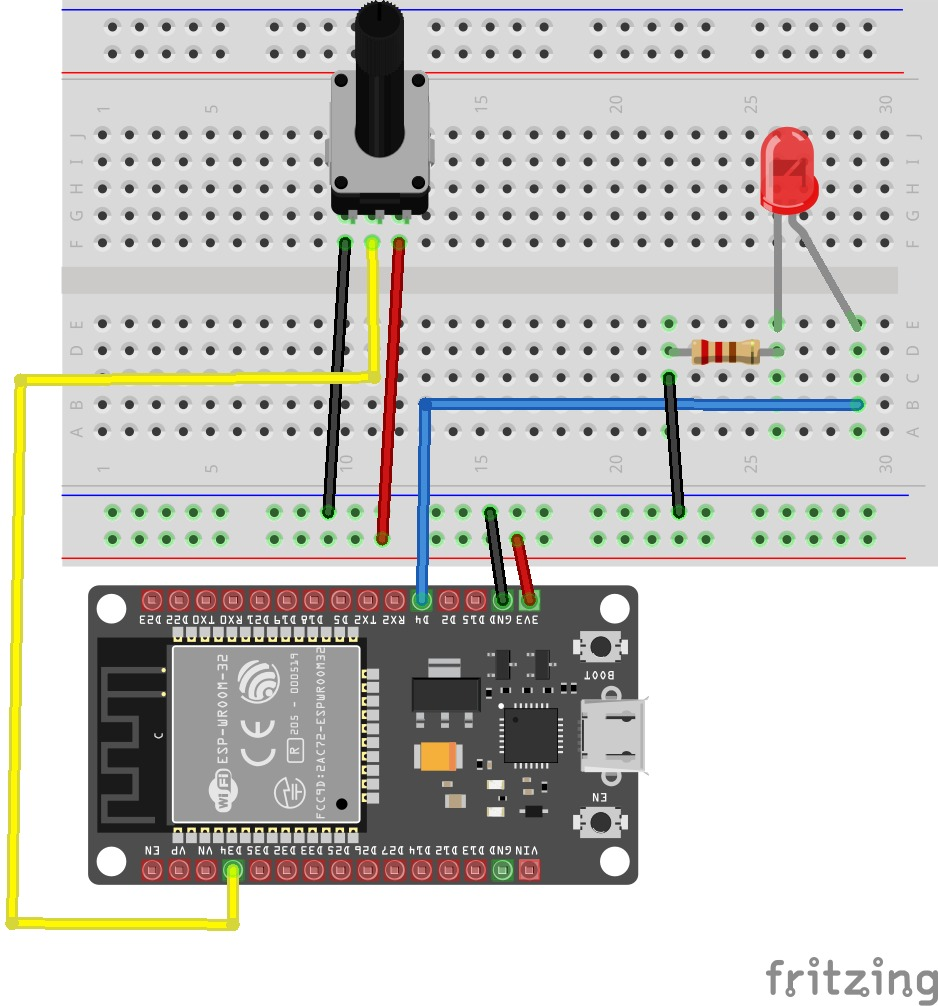
\includegraphics[width=0.85\textwidth]{../Esquemas/Potenciometro_esq.jpeg}
\caption{Esquema de conexión del circuito en Fritzing -- el WiFi es interno al ESP32}
\label{fig:esquema}
\end{figure}

\subsection{Diagrama de Conexiones}

\begin{center}
\begin{tabular}{lll}
\toprule
\textbf{Componente} & \textbf{Pin} & \textbf{ESP32 GPIO} \\
\midrule
Potenciómetro & Terminal 1 & 3.3V \\
Potenciómetro & Terminal 2 (cursor) & GPIO34 (ADC1\_CH6) \\
Potenciómetro & Terminal 3 & GND \\
Resistencia 220\,$\Omega$ & Terminal 1 & GPIO4 \\
LED & Ánodo (+) & Resistencia 220\,$\Omega$ (Terminal 2) \\
LED & Cátodo (--) & GND \\
\bottomrule
\end{tabular}
\end{center}

\textbf{Nota:} En este proyecto, la conectividad WiFi se utiliza exclusivamente para transmitir datos a la nube de ThingSpeak; el ESP32 no funciona como servidor web local, sino como \textbf{cliente HTTP} que envía información periódicamente a los servidores de MathWorks.

% ══════════════════════════════════════════════════════════════
\section{Código Fuente}
% ══════════════════════════════════════════════════════════════

A continuación se presenta el código completo del proyecto. Este programa combina la lectura de sensores analógicos con la comunicación IoT mediante la librería oficial de ThingSpeak.

\subsection{Código Completo}
\lstinputlisting[language=C++, title=Potenciometro\_ThingSpeak.ino]{../Arduino/Potenciometro_ThingSpeak/Potenciometro_ThingSpeak.ino}

% ══════════════════════════════════════════════════════════════
\subsection{Análisis del Código}
% ══════════════════════════════════════════════════════════════

El código se organiza en seis bloques de configuración claramente delimitados, seguidos de las funciones \texttt{setup()} y \texttt{loop()}.

\subsubsection*{Librerías Utilizadas}

\begin{itemize}
    \item \textbf{\texttt{WiFi.h}:} Proporciona las funciones para conectar el ESP32 a una red WiFi en modo estación (STA). Permite obtener la dirección IP asignada por DHCP y verificar el estado de la conexión.
    \item \textbf{\texttt{ThingSpeak.h}:} Librería oficial de MathWorks que simplifica la comunicación con la API de ThingSpeak. Permite configurar campos (\texttt{setField}), enviar múltiples campos en una sola petición HTTP (\texttt{writeFields}) y leer datos del canal.
\end{itemize}

\textbf{Instalación:} La librería ThingSpeak se instala desde el Gestor de Bibliotecas del Arduino IDE: \texttt{Programa $\rightarrow$ Incluir librería $\rightarrow$ Administrar bibliotecas $\rightarrow$} buscar ``ThingSpeak'' $\rightarrow$ instalar la versión de MathWorks.

\subsubsection*{Bloques de Configuración}

\begin{enumerate}
    \item \textbf{WiFi:} Se definen el SSID y la contraseña de la red (debe ser 2,4\,GHz).
    \item \textbf{ThingSpeak:} Se configuran el \texttt{Channel ID} (identificador numérico del canal) y la \texttt{Write API Key} (clave de 16 caracteres para autorizar escritura).
    \item \textbf{Pines:} GPIO34 para el potenciómetro (entrada analógica) y GPIO4 para el LED (salida digital).
    \item \textbf{Intervalo:} Se establece un período de 20\,000\,ms (20 segundos) entre envíos sucesivos.
    \item \textbf{Estado del LED:} Variable booleana \texttt{ledEncendido} que alterna en cada ciclo.
    \item \textbf{Cliente WiFi:} Objeto \texttt{WiFiClient} requerido por la librería ThingSpeak para las conexiones TCP.
\end{enumerate}

\subsubsection*{Función \texttt{setup()}}

\begin{enumerate}
    \item Inicia la comunicación serial a 115\,200 baudios.
    \item Configura GPIO34 como entrada y GPIO4 como salida (LED apagado).
    \item Conecta a la red WiFi con \texttt{WiFi.begin()} y espera hasta obtener \texttt{WL\_CONNECTED}.
    \item Imprime la dirección IP asignada al ESP32.
    \item Inicializa la comunicación con ThingSpeak mediante \texttt{ThingSpeak.begin(cliente)}.
\end{enumerate}

\subsubsection*{Función \texttt{loop()}}

El bucle principal utiliza un patrón \textbf{no bloqueante} con \texttt{millis()} en lugar de \texttt{delay()}, lo que permite que el procesador permanezca libre entre envíos:

\begin{enumerate}
    \item \textbf{Control de tiempo:} Si no han transcurrido 20\,s desde el último envío, retorna inmediatamente.
    \item \textbf{Lectura ADC:} Lee el potenciómetro con \texttt{analogRead()} (valor 0--4095).
    \item \textbf{Conversión a voltaje:} Aplica la fórmula:
    \begin{equation}
    V = \frac{\text{valorADC} \times 3{,}3}{4095}
    \label{eq:voltaje}
    \end{equation}
    \item \textbf{Alternancia del LED:} Invierte el estado booleano y actualiza GPIO4.
    \item \textbf{Preparación de campos:} Usa \texttt{ThingSpeak.setField(1, voltaje)} y \texttt{setField(2, estado)} para cargar los datos en un búfer temporal.
    \item \textbf{Envío:} Llama a \texttt{ThingSpeak.writeFields()} que transmite ambos campos en una sola petición HTTP POST al servidor de MathWorks. Retorna 200 si fue exitoso.
\end{enumerate}

% ══════════════════════════════════════════════════════════════
\section{Principio de Funcionamiento}
% ══════════════════════════════════════════════════════════════

\subsection{¿Qué es ThingSpeak?}

\textbf{ThingSpeak} es una plataforma IoT en la nube desarrollada por MathWorks (creadores de MATLAB). Permite:
\begin{itemize}
    \item \textbf{Recolectar datos} de dispositivos IoT a través de su API REST.
    \item \textbf{Almacenar} los datos en canales con hasta 8 campos (\textit{fields}).
    \item \textbf{Visualizar} los datos mediante gráficas temporales, gauges, indicadores y widgets personalizados.
    \item \textbf{Analizar} los datos con MATLAB integrado en la nube.
    \item \textbf{Compartir} los canales de forma pública o privada.
\end{itemize}

La cuenta gratuita permite un máximo de \textbf{1 escritura cada 15 segundos} por canal, razón por la cual el programa utiliza un intervalo de 20 segundos como margen de seguridad.

\subsection{Arquitectura del Sistema}

A diferencia de los proyectos anteriores donde el ESP32 actuaba como servidor (WiFi local) o transmisor directo (Bluetooth), en este proyecto el ESP32 funciona como \textbf{cliente HTTP} que envía datos a un servidor externo en Internet:

\begin{verbatim}
    Potenciómetro       ESP32            Internet          ThingSpeak
    (0 - 3.3 V)  ----> ADC 12-bit ----> HTTP POST ----> Servidor MathWorks
                        + LED toggle     WiFi             Almacena datos
                                                               |
                                                               v
                                                    Widgets de visualización:
                                                    - Field 1 Chart (voltaje)
                                                    - Gauge (potenciómetro)
                                                    - Lamp (estado del LED)
                                                               |
                                                               v
                                                    Navegador / App móvil
                                                    (acceso desde cualquier
                                                     lugar del mundo)
\end{verbatim}

\subsection{Configuración del Canal ThingSpeak}

Para utilizar este proyecto, es necesario configurar un canal en ThingSpeak con los siguientes pasos:

\begin{enumerate}
    \item Crear una cuenta gratuita en \url{https://thingspeak.mathworks.com}.
    \item Crear un nuevo canal (\textit{New Channel}) con dos campos:
    \begin{itemize}
        \item \textbf{Field 1:} Potenciómetro (almacena el voltaje en voltios).
        \item \textbf{Field 2:} LED (almacena el estado: 1 = encendido, 0 = apagado).
    \end{itemize}
    \item En la pestaña \textit{API Keys} del canal, copiar:
    \begin{itemize}
        \item \textbf{Channel ID:} Número identificador del canal.
        \item \textbf{Write API Key:} Clave de 16 caracteres para autorizar la escritura de datos.
    \end{itemize}
    \item Agregar widgets de visualización: gráfica temporal para Field~1, gauge para el voltaje y lámpara para el estado del LED.
\end{enumerate}

\subsection{Protocolo de Comunicación}

La librería ThingSpeak encapsula la siguiente secuencia de comunicación HTTP:

\begin{enumerate}
    \item El ESP32 establece una conexión TCP con \texttt{api.thingspeak.com} en el puerto 80.
    \item Construye una petición HTTP POST con los campos configurados.
    \item Incluye la \textit{Write API Key} como cabecera de autenticación.
    \item El servidor recibe los datos, los almacena con marca temporal y retorna un código de estado.
\end{enumerate}

Los códigos de respuesta más comunes son:

\begin{center}
\begin{tabular}{cl}
\toprule
\textbf{Código} & \textbf{Significado} \\
\midrule
200 & Datos recibidos correctamente \\
$-$301 & Error de conexión (verificar WiFi) \\
$-$401 & API Key incorrecta \\
$-$210 & Campo no válido \\
\bottomrule
\end{tabular}
\end{center}

\subsection{El Potenciómetro como Divisor de Voltaje}

El potenciómetro actúa como divisor de voltaje ajustable. Con sus terminales extremos entre 3,3\,V y GND:

\begin{equation}
V_{\text{cursor}} = V_{CC} \times \frac{\theta}{\theta_{\max}} = 3{,}3 \times \frac{\theta}{270°}
\label{eq:divisor}
\end{equation}

El ADC de 12 bits del ESP32 digitaliza este voltaje con una resolución de:
\begin{equation}
\Delta V = \frac{3{,}3\,\text{V}}{4095} \approx 0{,}806\,\text{mV por paso}
\end{equation}

% ══════════════════════════════════════════════════════════════
\section{Fotografías del Montaje}
% ══════════════════════════════════════════════════════════════

Las siguientes imágenes documentan el proyecto en funcionamiento, mostrando tanto el dashboard de ThingSpeak en la nube como el montaje físico del circuito.

\begin{figure}[H]
\centering
\begin{subfigure}[b]{0.48\textwidth}
    \centering
    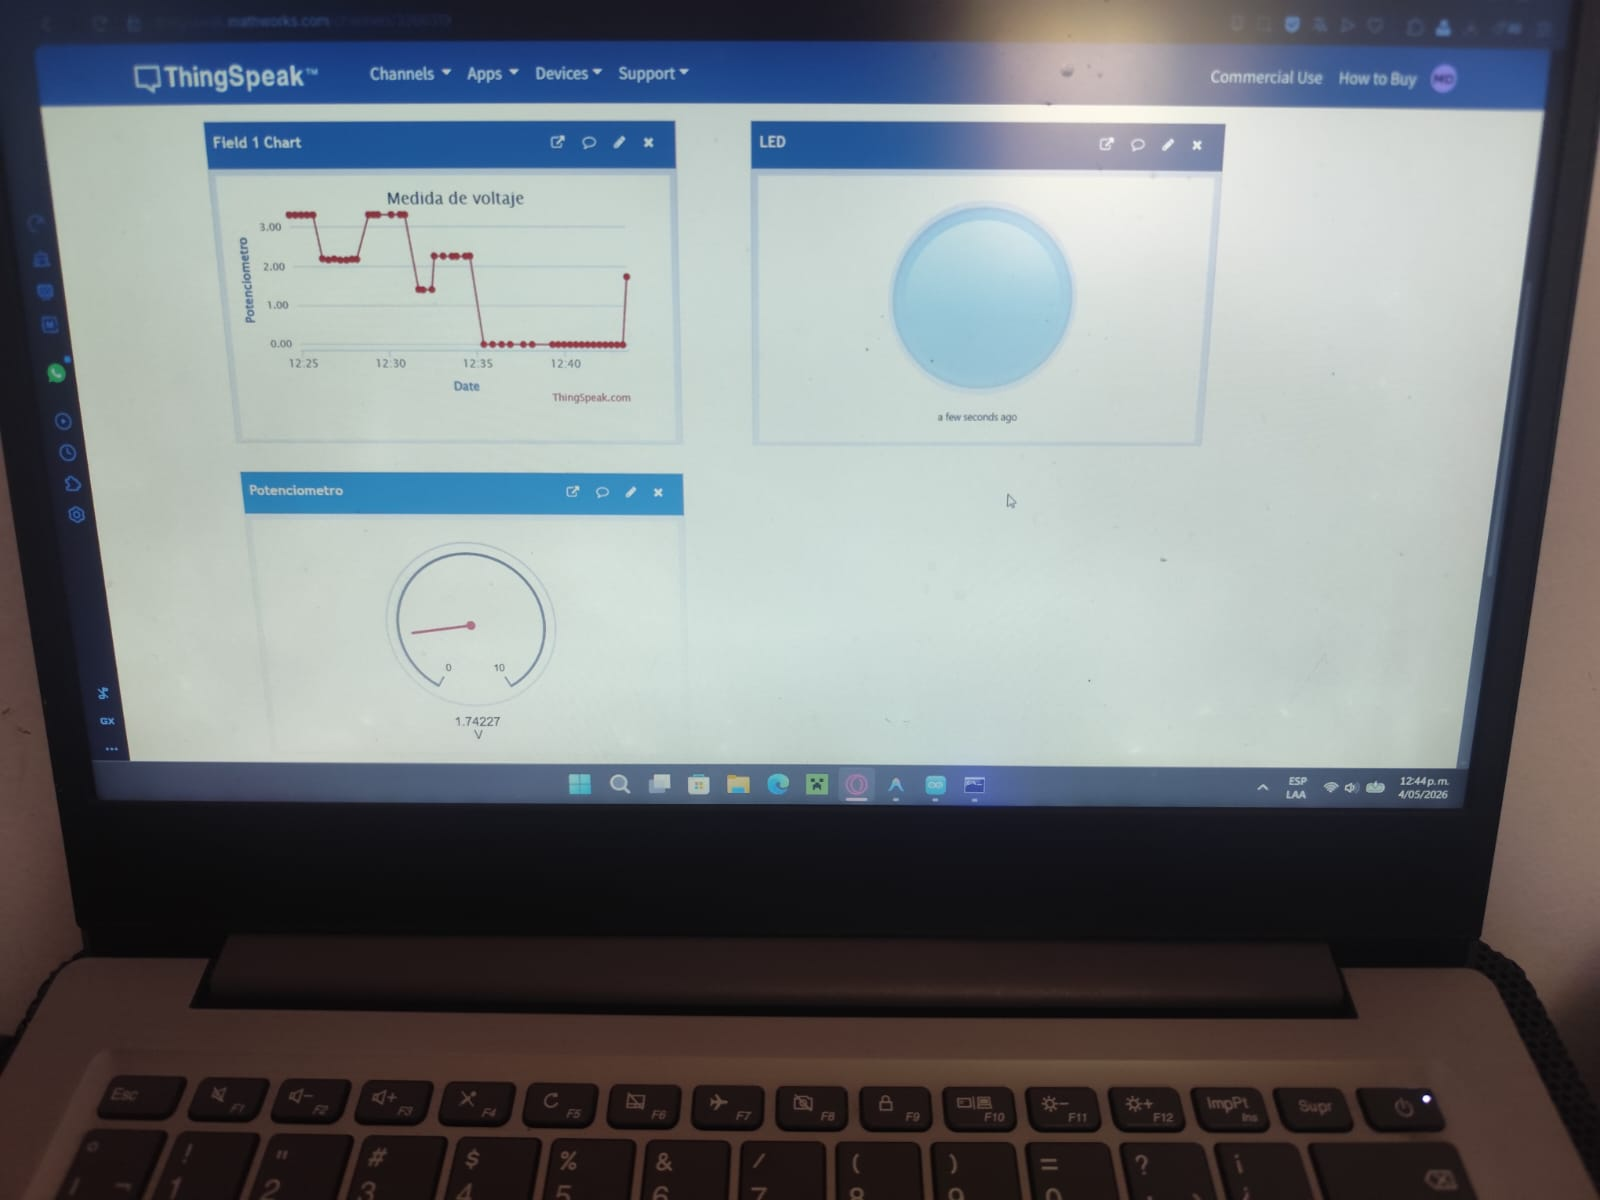
\includegraphics[width=\textwidth]{../Imagenes/Potenciometro_ThingSpeak_imgs/Potenciometro_ThingSpeak_img1.jpeg}
    \caption{Dashboard de ThingSpeak en el navegador del computador. Se observan tres widgets: (1) \textit{Field 1 Chart} con la gráfica temporal del voltaje del potenciómetro mostrando variaciones entre 0 y 3\,V, (2) widget de lámpara ``LED'' indicando el estado actual, y (3) gauge ``Potenciómetro'' marcando 1,74\,V.}
    \label{fig:thingspeak1}
\end{subfigure}
\hfill
\begin{subfigure}[b]{0.48\textwidth}
    \centering
    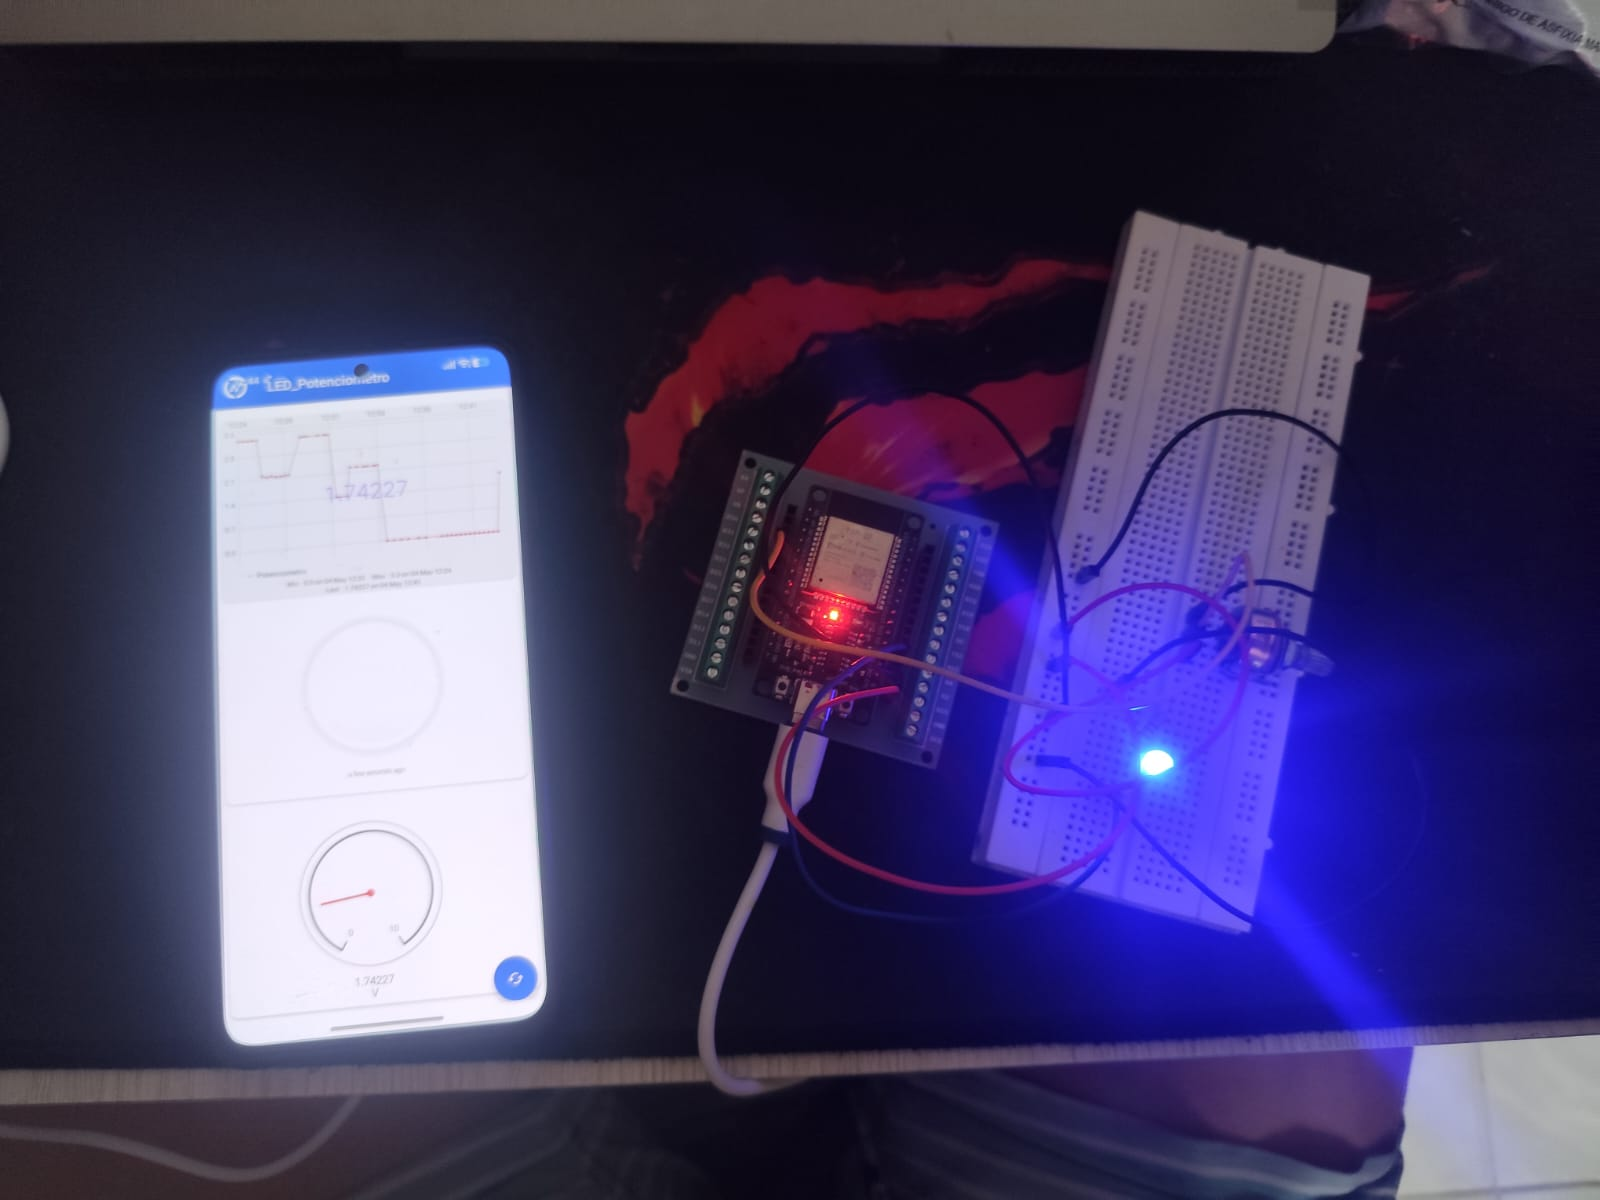
\includegraphics[width=\textwidth]{../Imagenes/Potenciometro_ThingSpeak_imgs/Potenciometro_ThingSpeak_img2.jpeg}
    \caption{Vista del montaje físico: celular mostrando la app de ThingSpeak con los mismos datos del dashboard (gráfica, lámpara y gauge a 1,74\,V), junto al ESP32 conectado a la protoboard con el LED encendido en azul y el potenciómetro visible.}
    \label{fig:thingspeak2}
\end{subfigure}
\caption{Dashboard de ThingSpeak y montaje físico del proyecto}
\label{fig:montaje}
\end{figure}

En las Figuras~\ref{fig:thingspeak1} y~\ref{fig:thingspeak2} se puede observar:
\begin{itemize}
    \item La gráfica temporal (\textit{Field 1 Chart}) muestra el historial de lecturas del potenciómetro con marcas temporales, permitiendo visualizar cómo el usuario giró la perilla a lo largo del tiempo.
    \item El widget de lámpara cambia de color según el estado del LED: encendido (azul claro) o apagado.
    \item El gauge analógico muestra el voltaje actual del potenciómetro en una escala de 0 a 10\,V, con la lectura numérica 1,74227\,V debajo.
    \item El mismo canal es accesible simultáneamente desde el computador (navegador web) y desde el celular (aplicación móvil de ThingSpeak), demostrando la naturaleza cloud del sistema.
    \item En la imagen del montaje físico se aprecia el ESP32 con su LED de estado, el LED azul del circuito encendido, el potenciómetro y las conexiones en la protoboard.
\end{itemize}

% ══════════════════════════════════════════════════════════════
\section{Videos de Funcionamiento}
% ══════════════════════════════════════════════════════════════

Se dispone de un video que demuestra el funcionamiento completo del proyecto:

\begin{itemize}
    \item \textbf{Potenciometro\_ThingSpeak\_Funcionamiento.mp4}: Demostración del sistema en funcionamiento, mostrando cómo al girar el potenciómetro y esperar el ciclo de 20 segundos, los datos se actualizan automáticamente en el dashboard de ThingSpeak. Se observa la sincronización entre el circuito físico (LED alternando) y los widgets en la nube (gráfica actualizándose, gauge moviéndose, lámpara cambiando de estado).
\end{itemize}

Este video se encuentra en la carpeta \texttt{Videos/Potenciometro\_ThingSpeak\_vid/} del repositorio del proyecto.

% ══════════════════════════════════════════════════════════════
\section{Proceso de Creación}
% ══════════════════════════════════════════════════════════════

El desarrollo de este proyecto partió de los conceptos de los proyectos anteriores y añadió la capacidad de enviar datos a la nube:

\begin{enumerate}
    \item \textbf{Punto de partida:} Se reutilizó el circuito del potenciómetro y LED de los proyectos anteriores, cambiando únicamente el software.
    
    \item \textbf{Creación del canal ThingSpeak:} Se creó una cuenta gratuita en ThingSpeak y se configuró un canal con dos campos (voltaje y estado del LED), obteniendo el Channel ID y la Write API Key.
    
    \item \textbf{Instalación de la librería:} Se instaló la librería oficial ``ThingSpeak'' de MathWorks desde el gestor de bibliotecas del Arduino IDE.
    
    \item \textbf{Programación del firmware:} Se escribió el código que conecta al WiFi, lee el potenciómetro, alterna el LED y envía ambos datos a ThingSpeak usando \texttt{setField()} y \texttt{writeFields()}.
    
    \item \textbf{Configuración de widgets:} En el dashboard de ThingSpeak se agregaron tres widgets de visualización: gráfica temporal para el voltaje, gauge analógico para la lectura actual, y lámpara indicadora para el estado del LED.
    
    \item \textbf{Pruebas y validación:} Se verificó que los datos llegaran correctamente observando la gráfica en tiempo real y confirmando que el código de respuesta fuera 200 en el monitor serial.
\end{enumerate}

% ══════════════════════════════════════════════════════════════
\section{Diferencias con Proyectos Anteriores}
% ══════════════════════════════════════════════════════════════

\begin{table}[H]
\centering
\begin{tabular}{lcccc}
\toprule
\textbf{Característica} & \textbf{Base} & \textbf{Bluetooth} & \textbf{WiFi Local} & \textbf{ThingSpeak} \\
\midrule
Lectura ADC & \checkmark & \checkmark & \checkmark & \checkmark \\
Control del LED & PWM & PWM & On/Off web & Auto-toggle \\
Monitoreo serial & \checkmark & \checkmark & Depuración & Depuración \\
Comunicación & USB & BT SPP & WiFi HTTP & WiFi + nube \\
Interfaz de usuario & Terminal & App BT & Página web & Dashboard cloud \\
Acceso remoto & -- & -- & Red local & Internet global \\
Almacenamiento datos & -- & -- & -- & \checkmark (nube) \\
Historial temporal & -- & -- & En sesión & Persistente \\
\bottomrule
\end{tabular}
\caption{Comparación entre los cuatro proyectos de potenciómetro}
\end{table}

% ══════════════════════════════════════════════════════════════
\section{Conceptos Técnicos Clave}
% ══════════════════════════════════════════════════════════════

\subsection{IoT y Computación en la Nube}

El \textbf{Internet de las Cosas (IoT)} se refiere a la interconexión de dispositivos físicos con Internet para recolectar, transmitir y analizar datos. ThingSpeak es un ejemplo de plataforma \textbf{IoT como Servicio (IoTaaS)} que abstrae la complejidad de servidores, bases de datos y visualización, permitiendo al desarrollador enfocarse en el firmware del dispositivo.

\subsection{API REST de ThingSpeak}

ThingSpeak expone una API RESTful donde cada canal tiene URLs específicas para lectura y escritura. La librería oficial encapsula estas llamadas, pero internamente realiza peticiones HTTP POST a:
\begin{verbatim}
    POST https://api.thingspeak.com/update
    Content-Type: application/x-www-form-urlencoded
\end{verbatim}

\subsection{Patrón No Bloqueante con \texttt{millis()}}

El código utiliza \texttt{millis()} en lugar de \texttt{delay()} para controlar el intervalo de envío. Este patrón permite que el procesador permanezca disponible para otras tareas durante los 20 segundos entre envíos, en lugar de quedar bloqueado.

\subsection{Campos Múltiples en Una Sola Petición}

ThingSpeak limita a 1 escritura cada 15 segundos por canal, no por campo. Por eso el código usa \texttt{setField()} para preparar ambos campos y luego \texttt{writeFields()} para enviarlos juntos en una sola petición HTTP, optimizando el uso del ancho de banda.

% ══════════════════════════════════════════════════════════════
\section{Conclusiones}
% ══════════════════════════════════════════════════════════════

\begin{itemize}
    \item El proyecto demuestra cómo integrar el ESP32 con la plataforma IoT ThingSpeak para enviar datos a la nube y visualizarlos remotamente desde cualquier dispositivo con acceso a Internet.
    \item La librería oficial de ThingSpeak simplifica enormemente la comunicación con la API REST, reduciendo el código de red a pocas líneas (\texttt{begin}, \texttt{setField}, \texttt{writeFields}).
    \item El uso del patrón no bloqueante con \texttt{millis()} mantiene el procesador disponible entre envíos, a diferencia de \texttt{delay()} que detiene toda ejecución.
    \item Los widgets de ThingSpeak (gráfica temporal, gauge y lámpara) proporcionan una visualización profesional sin necesidad de desarrollar una interfaz web propia.
    \item El almacenamiento persistente en la nube permite revisar el historial de datos incluso después de apagar el ESP32, algo imposible con los proyectos anteriores.
    \item El acceso simultáneo desde computador y celular (demostrado en las fotografías) confirma la naturaleza verdaderamente distribuida del sistema IoT.
    \item Este proyecto representa la evolución natural de los proyectos anteriores: de local (USB) a inalámbrico cercano (Bluetooth), a red local (WiFi) y finalmente a Internet global (ThingSpeak/nube).
\end{itemize}

\end{document}
